\Chapter{Képek közelítése a bemeneti vektorok terében}

A GAN által betanult térről nem kapunk egzakt információkat, nincs tudomásunk arról, hogy a modell hogyan helyezte el a sokdimenziós térben a tanult ismereteit. Egy betanított modell esetén csupán annyit látunk, hogy különböző random bemeneti vektorokra különböző képeket kapunk a generátor kimenetén.
Két random zajvektor között ha interpolálunk, akkor minden egyes mintavételezett pontból ki tudunk generálni olyan képeket, amelyek a két kép közti átmenetet jelentik és amelyeken megfigyelhetőek a két kép együttes tulajdonságai. A \ref{fig:interpolation} ábrán látható egy példa az interpolációra.

\begin{figure}[h]
\centering
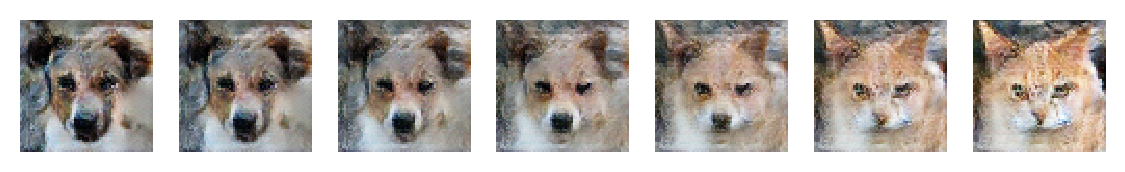
\includegraphics[width=15cm]{images/interpolation.png}
\caption{Generált képek lineáris interpolációval két zajvektor között}
\label{fig:interpolation}
\end{figure}

A bemeneti vektorok tere tehát folytonosan van kitöltve, bármely pontra egy képet kaphatunk vissza. Viszont ezen tér feltérképezése sem egy triviális feladat és az sem biztosított, hogy a tér az egymáshoz hasonló jellegzetességekkel van kitöltve.

A képek közelítésre egy megoldás lehet a \textit{synthesis-through-optimization}\cite{frans2021clipdraw} technika, amelyhez nem kell betanítani egy újabb modellt, csupán optimalizációs alapon történik meg a képek közelítése.
A technikához szükségünk van egy célfüggvényre, amelyre az optimalizációt végre tudjuk hajtani egy megjelenítőre, amely esetünkben a GAN generátora lesz és egy olyan eszközre, amellyel mérni tudjuk a kigenerált képek jóságát. Az utóbbi eszköz általában egy osztályozó szokott lenni, amelynek a tudásával bejárhatjuk a vizsgált teret. Az optimalizálást pedig a gradiens keresés módszerével szokás végrehajtani.
A CLIP \cite{radford2021learning} zero-shot osztályozó igen közkedvelt az ilyen fajta vizsgálatok elvégzésére. Az osztályozó kimenetén szabad szöveges mondatok jelennek meg a vizsgált képekre a megfelelő valószínűségi értékekkel kiegészítve. A CLIPDraw-ban \cite{frans2021clipdraw}  például nem is GAN modellt használtak a képek generálására, hanem csupán Bézier-görbék halmazán végezték el az optimalizálást és eredményül rajzokhoz hasonló képeket kaptak. Esetükben a célfüggvény a bemeneti mondatok és a CLIP osztályozó által kiadott mondat koszinuszi távolságának minimalizálása volt. A keresés végén a görbék olyan alakban rendeződtek, amelyek legjobban reprezentálják a bemeneti szabad-szöveges mondatot a CLIP osztályozó szerint.

A GAN $G$ generátorának bemenete egy $\vec{z} \in \mathbb{R}^{z_n}$ vektor, ahol $z_n$ általában 100 szokott lenni. Vagyis a bemeneti vektor egy $z_n$ dimenziójú tér egy pontja. A 100 dimenzióban történő keresés igen nehéz lehet a hagyományos heurisztikus módszerekkel, mint például a hegymászó módszerrel. A hegymászó optimalizáló módszer során a célfüggvényt minimalizáljuk (vagy maximalizáljuk) a pont körüli tartomány mintavételezésével, majd a megfelelő szomszédos pontra való lépéssel. A bemeneti paraméter lehet a pont kiinduló pozíciója, a lépésköz és a mintavételezés sűrűsége. A megfelelő pontosság érdekében igen sok mintára lehet szükségünk és ez egy sokdimenziós térben igen nagy lehet. A módszer hátránya lehet a fix lépésköz is, amely hatására lokális optimumokban ragadhatunk, ha a vizsgált felületünk bonyolult. Több vizsgálandó pont elszórása a térben megnövelheti az esélyét annak, hogy rátalálunk a globális optimumra is, viszont ez jelentősen megnöveli a számításigényt.
A gradiens módszer vagy gradient süllyesztés (\textit{Gradient Descent}) egy olyan iteratív optimalizáló módszer, amely a diferenciálható függvény lokális minimumának megtalására irányul. A célfüggvény elsőrendű deriváltjai igazítják el a vizsgált pontunkat a minimumhoz.

Egy kiválasztott kép közelítése a bemeneti vektorok terében az alábbi módon történhet:\\ 
Jelölje $X$ a keresendő képet, $G$ a generátort, $\vec{z} \in \mathbb{R}^{z_n}$ pedig a látens vektort.\\
A cél egy olyan $\vec{z} \in \mathbb{R}^{z_n}$ látens vektor keresése, amellyel az alábbi távolság minimalizálható.

$$ \min\left(\sum_{i=1}^{n\times m}\sqrt{(X_i-G(\vec{z})_i)^2}\right)$$

A képeket tehát pixelszinten hasonlítjuk össze kiindulásképp. Ez a távolságot szokás L2 távolságnak is nevezni, az L2 norma alapján, vagy euklideszi távolságnak is.
Egyéb metrikákat is alkalmazhatunk a képek hasonlóságának mérésére, ilyen a PCA, a HOG, MSE, stb...

Legyen $l$ a lépésméret, $X \in \mathbb{R}^{n\times m \times 3}$ a keresendő kép, $G$ pedig a betanított generátor.
\begin{enumerate}
	\item Generáljunk egy képet az aktuális $\vec{z}$ zajvektorral
$$\hat X = G(\vec{z})$$
	\item Számoljuk ki a generált kép és a keresendő kép távolságát.
$$ loss = \sum_{i=1}^{n\times m}\sqrt{(X_i-\hat X_i)^2} $$
	\item Számoljuk ki a gradienseket a hibafüggvény szerint
$$ \vec{grad} = \frac{d}{d\vec{z}} \left[loss\right]$$
	\item Módosítsuk a $\vec{z}$ zajvektor elemeit a kapott gradiensek szerint egy $l$ hosszúságú lépéssel
$$ z_i = z_i - (l \cdot grad_i)$$
	\item Ismételjük meg az algoritmust a konvergálásig.
\end{enumerate}

Azt, hogy pontosan mikor kell befejeznünk az algoritmust nincsen meghatározva előre. A hibafüggvények változát esetleg nyomon követhetnénk, és ha két érték között oszcillál a hibafüggvény, akkor valószínűleg elért az algoritmus egy lokális minimumot. A példa egyszerűsítése kedvéért a lépésszám is egy bemeneti paraméter jelen esetben.

Az algoritmus Tensorflow-ban történő megvalósítása a következő:

\begin{python}
random_noise = tf.random.uniform([1, latent_dim], minval=-1, maxval=1)
noise = tf.Variable(random_noise)
step_size = 0.03
steps = 50
for i in range(steps):
    with tf.GradientTape() as g_tape:
        g_tape.watch(noise)
        generated_image = generator(noise, training=False)
        loss = tf.norm(goal_image - generated_image)
    gradients = g_tape.gradient(loss, noise)
    noise = noise - (step_size * gradients)
\end{python}


Momentummal való kiegészítés:

Jelöljük $t$-vel az időpillanatot.

$$ z_i^t = z_i^{t-1} - (l \cdot f'(z_i^{t-1})$$

$$ valtozas^t = l \cdot f'(z_i^{t-1}) $$

$$ z_i^t = z_i^{t-1} - valtozas^t $$


Momentum esetén a változás:
$$ valtozas^t = l \cdot f'(z_i^{t-1}) + momentum \cdot valtozas^{t-1}$$


momentum 0 - 1 között (0 esetén sima gradient descent)


\begin{figure}[h]
\centering
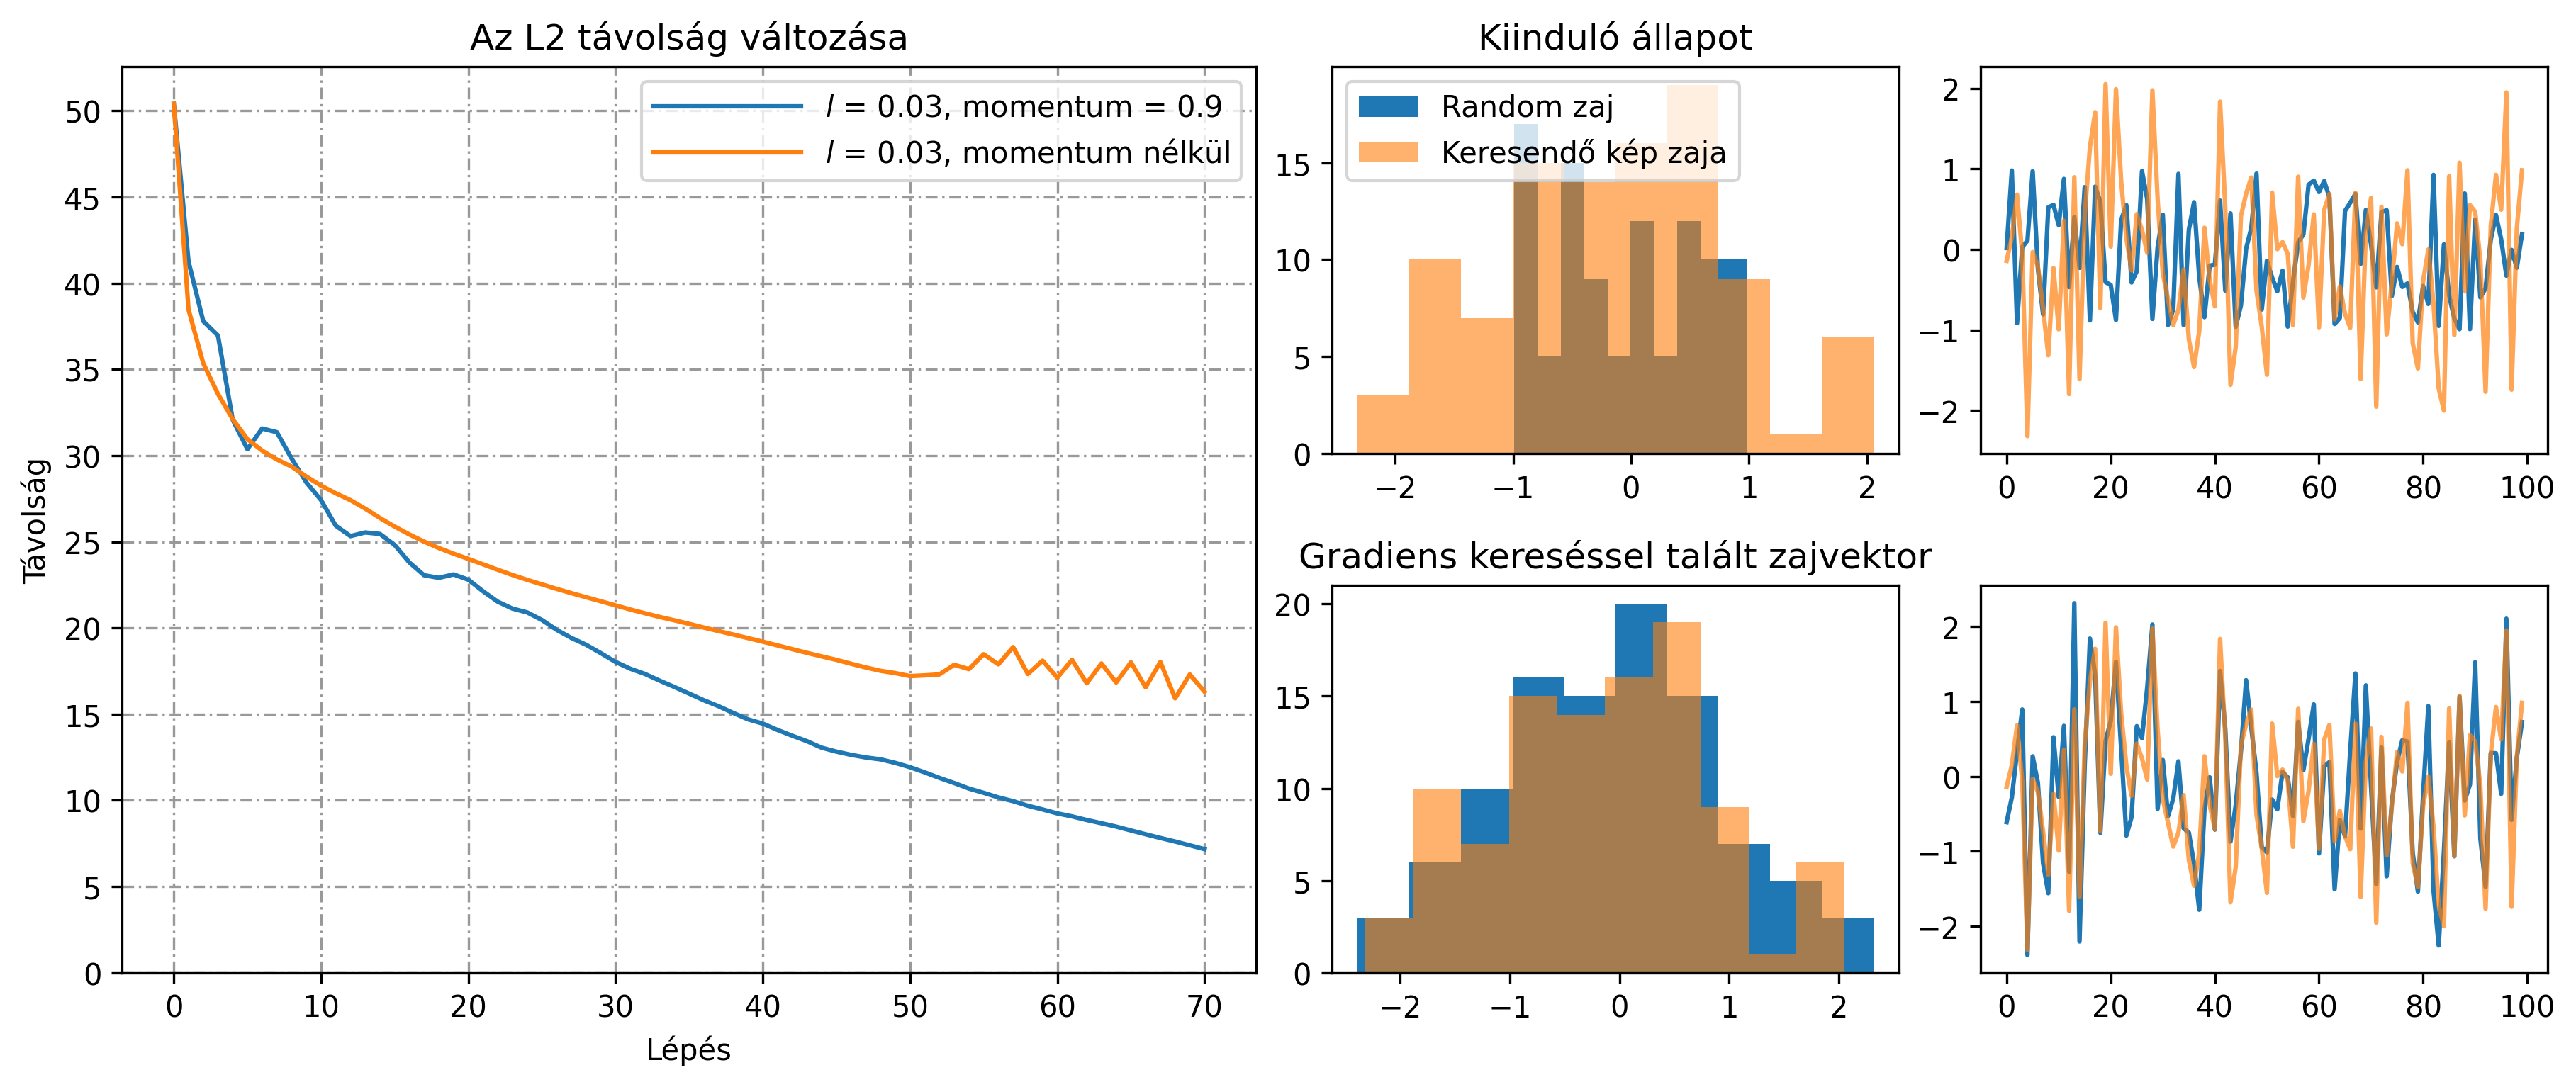
\includegraphics[width=15cm]{images/grad_losses.png}
\caption{A hibafüggvény változása a lépések során}
\label{fig:gradlosses}
\end{figure}


\begin{figure}[h]
\centering
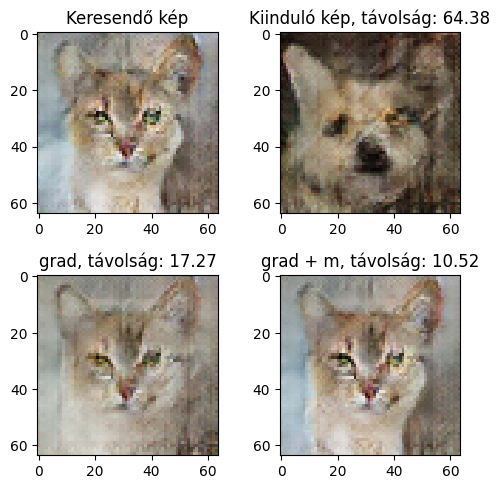
\includegraphics[width=8cm]{images/grad_found.png}
\caption{Gradiens kereséssel visszakeresett képek}
\label{fig:gradfound}
\end{figure}


\Section{Minták klaszterezése}

A GAN tanítása során a generátor a bemeneti vektorok terére megtanulja, hogy a tér egyes pontjaira milyen adatot képezzen le. A térből mintavételezett adatok mindegyikére egy, a tanítóhalmaz eloszlását követő adatot tud kigenerálni.
A tanítási lépések során általában a Normális vagy Egyenletes eloszlás szerint generálunk pontokat és azok alapján tanul a generátor modellunk. Annak ellenére, hogy a tér egyes pontjaira igen jól betanul a modell, nem garantálható, hogy az így keletkezett tér megfelelően klaszterezhető lehet és valójában a tanítás során generált pontok eloszlását követik a klaszterek pontjai \cite{mukherjee2019clustergan}.

Thus even though the latent
space may contain full information about the data, the dis-
tance geometry in the latent space does not reflect the inher-
ent clustering

\SubSection{Tanítás címkékkel}

A GAN alap esetben minták rendezetlen halmazán tanul. Viszont a legtöbb adathalmaz annotációkkal van ellátva, amelyeket így nem veszünk figyelembe a tanítás során és a modellre bízzuk, hogy megtanulja reprezentálni a tanítóhalmaz különféle objektumait. Ha szempont, hogy a GAN különféle osztályokra tudjon képeket generálni, akkor használhatjuk a Class Conditioning technikát \cite{mirza2014conditional}. Ezzel a modellnek egyfajta könnyítést is adhatunk a tanulás során, ha olyan adathalmazra végezzük el a tanítást, amely többfajta osztály objektumait tartalmazza. A technika alkalmazásával a modellünk nem a teljes adathalmazra próbál általánosítást találni, csupán az egyes osztályokra, ezzel is megkönnyítve a tanítást.

Egyes eredményeknél megfigyelhető, hogy a tanítás során az adathalmaz tisztítására is nagy gondot fordítottak. Például az olyan GAN modelleknél, amelyeknél a felbontás növelését tűzték ki megoldandó problémaként. Az ilyen modelleknél egy széles körben alkalmazott adathalmaz a CELEB FACES, amely hollywoodi hírességek portréit tartalmazza. Az említett adathalmazt erősen módosították a szerzők, például a szemeket és az egyéb arci jellegzetességeket pozícionálták minden egyes elemnél.

Ha a modellt olyan datasetre tanítjuk, amelyben hasonló objektumok találhatóak, akkor az így betanított GAN-okat domén-specifikusnak is nevezhetünk, hiszen a tudása csupán egy-egy osztály objektumaira korlátozódik. Egy-egy valós obejktumok többféleképpen is le tudunk fényképezni és ezáltal leképezni egy két dimenziós térre, így a GAN modellnek az is segítség lehet, ha csak olyan képeket mutatunk neki a tanítás során, amelyeket fix pozíciókból fényképeztünk.
Ilyen például a már említett hírességek portréit tartalmazó dataset is, amelyben csupán emberekről tartalmaz képeket és a legtöbb esetben a személy teljesen szemben áll a kamerával és rajta kívül nem látszik más a képen. Az általánosítás szempontjából ez egy nagy könnyítés lehet a modellnek.

A fotorealisztikus eredményeket elérő modellek esetén kijelenthetjük, hogy nagy szerepe van a megfelelő adathalmaznak is. Továbbá az ilyen jellegű cikkeknél a data-augmentation technikák használata is előfordul. Az eredmények reprodukálása tehát igen sok mozgó paramétertől függhet.

A class-conditioning technika alkalmazása során a generátor és a diszkriminátor egyszerre kerül kondicinálásra, vagyis minden egyes tanítási lépésnél a kondicionáló címkék meg fognak egyezni. Viszont a tanítás során nem ellenőrizzük le, hogy valóban helyesen lettek-e kondicionálva, hiszen továbbra is a megszokott kimenetekkel fog rendelkezni a generátor és a diszkriminátor is.

A hibafüggvény a következőképpen írható fel:

$$\min_{G}\max_{D}V(D, G) =  \mathbb{E}_{x \sim P(x)} \left[\ln D(x|y) \right] + \mathbb{E}_{z \sim P(z)} \left[\ln(1 - D(G(z|y))) \right]$$

Egy-egy tanítási lépés során a generátor és a diszkriminátor is ugyan azt az $y$ címkét kapja bemenetként (Illetve a diszkriminátor $y$ címkéhez tartozó valós képeket).

Az architektúrát minkét oldalon módosítani kell. A technikát felvázoló cikkben \cite{mirza2014conditional} kiemelték, hogy a $P(z)$ zajvektor és az $y$ címke kombinálására vaonatkozólag a GAN keretrendszer igen rugalmas tud lenni. A rugalmasság a kombinálásra is vonatkozhat, a szerzők nem is kötötték meg, hogy milyen módon lehet összeilleszteni a $z$-t és $y$-t. Én az egyszerűség kedvéért egy multiply réteget választottam, hiszen így nem változik a bemeneti dimenziószám és a kondicionálást a generátor elején el lehet végezni. Viszont meg lehet fontolni több komponáló módot is, mint például a konkatenációt, vagy az add réteg használatát is. (Ki lehetne próbálni...)

A $y$ címke a Cifar-10 adathalmaz esetében egy egész szám, amely 0 és 9 közötti értéket vehet fel. Az $y$ címkét egy \textit{embedding} réteg segítségével egy, a látens dimenzióval megegyező vektorrá alakítjuk, majd a $z$ zajvektorral való összeszorzás (vagy concat) előtt egy flattening réteggel a megfelelő formára hozzuk a kimeneti tensort.
A \textit{multiply} réteg segítségével összeszorzásra kerül az vektorizált címke és a zajvektor, amelynek kimenete lesz a generátor modellünk bemenete. A generátor modell felépítése megegyezik a már ismert, korábban felvázolt generátor architektúrájával. 

\begin{figure}[h]
\centering
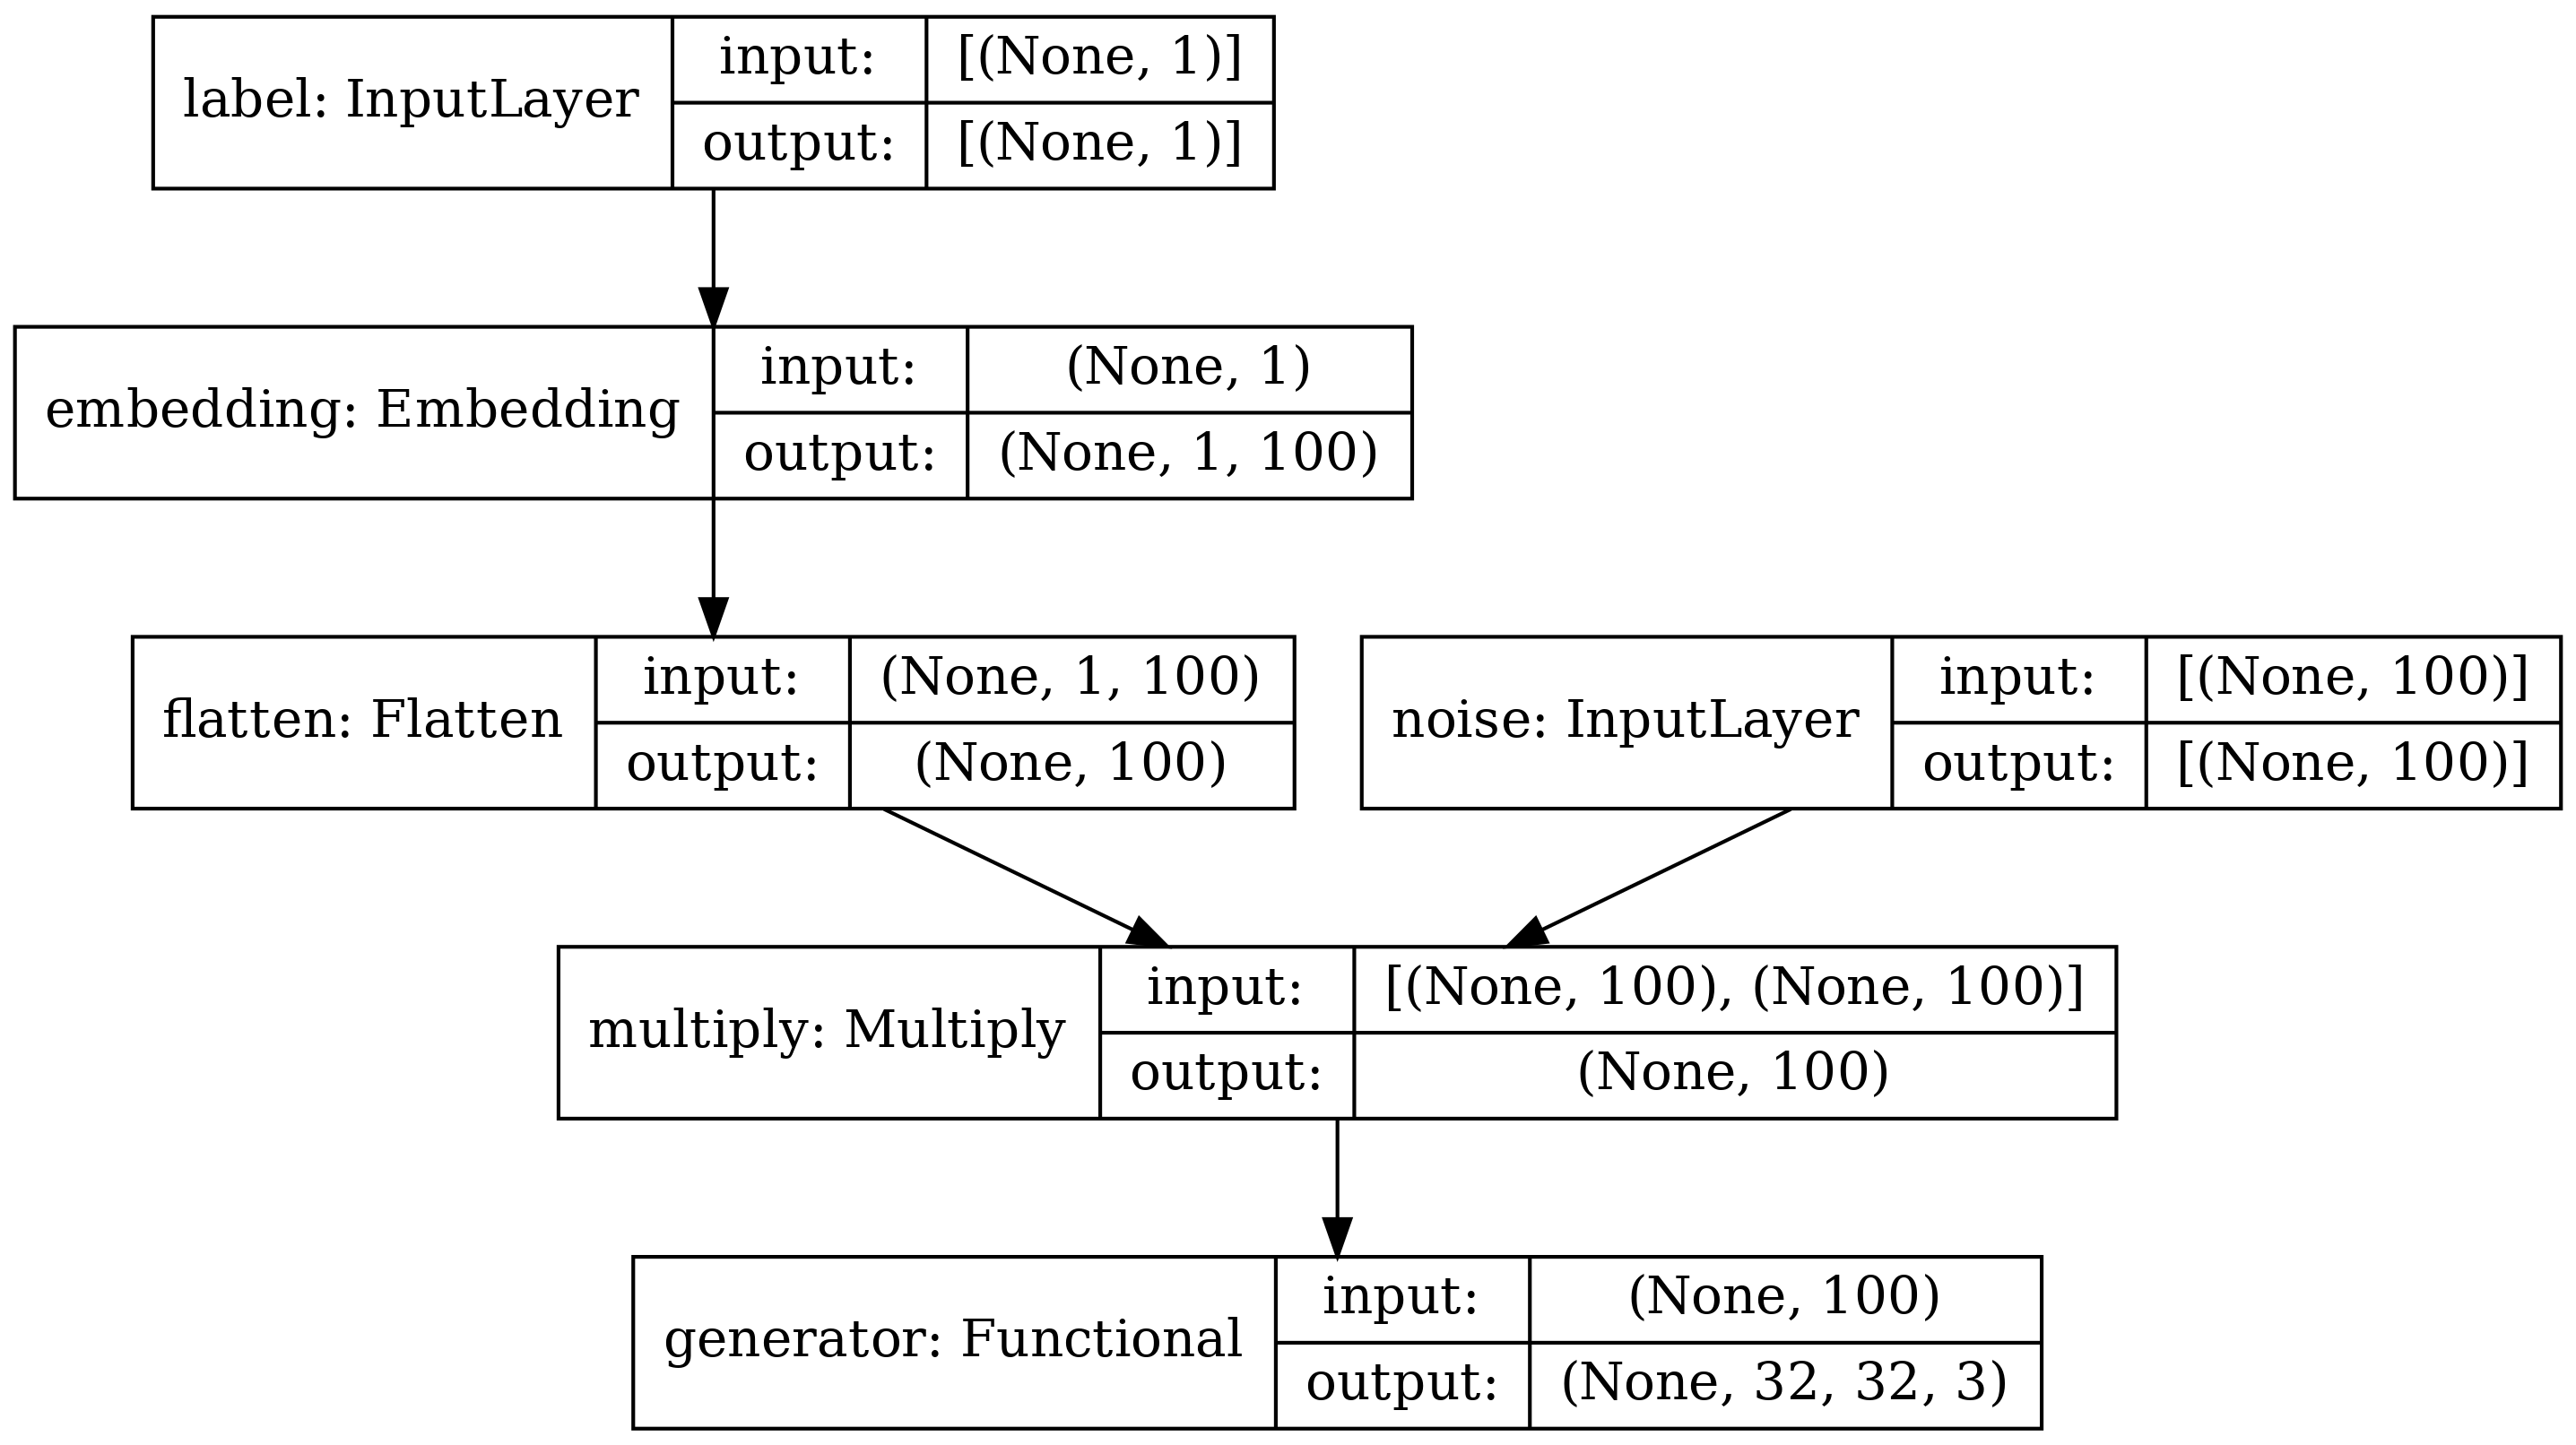
\includegraphics[width=13cm]{images/label_noise_embedding.png}
\caption{A zajvektor és a címke összeállítása a generátor bemeneteként}
\label{fig:labelnoiseembedding}
\end{figure}

A diszkriminátorban a kondicionálást a modell belsejében hajtom végre. Mivel a diszkriminátorunk a generátor tükörképének is tekinthető, így a diszkriminátor esetén nem a képpel együtt kerül be a címke a modellbe, hanem a modell által kinyert belső reprezentációkkal kerül összeszorzásra a címkét reprezentáló vektor, az utolsó teljesen összekapcsolt réteg előtt. A label conditioning technikát felvető cikkben megemlítették a \textit{dropout} réteg használatát is, így a teljesen összekapcsolt réteg előtt beillesztettem egy olyan réteget is.
A diszkriminátor felépítése a \ref{fig:labeldiscriminator} ábrán látható.

\begin{figure}[h]
\centering
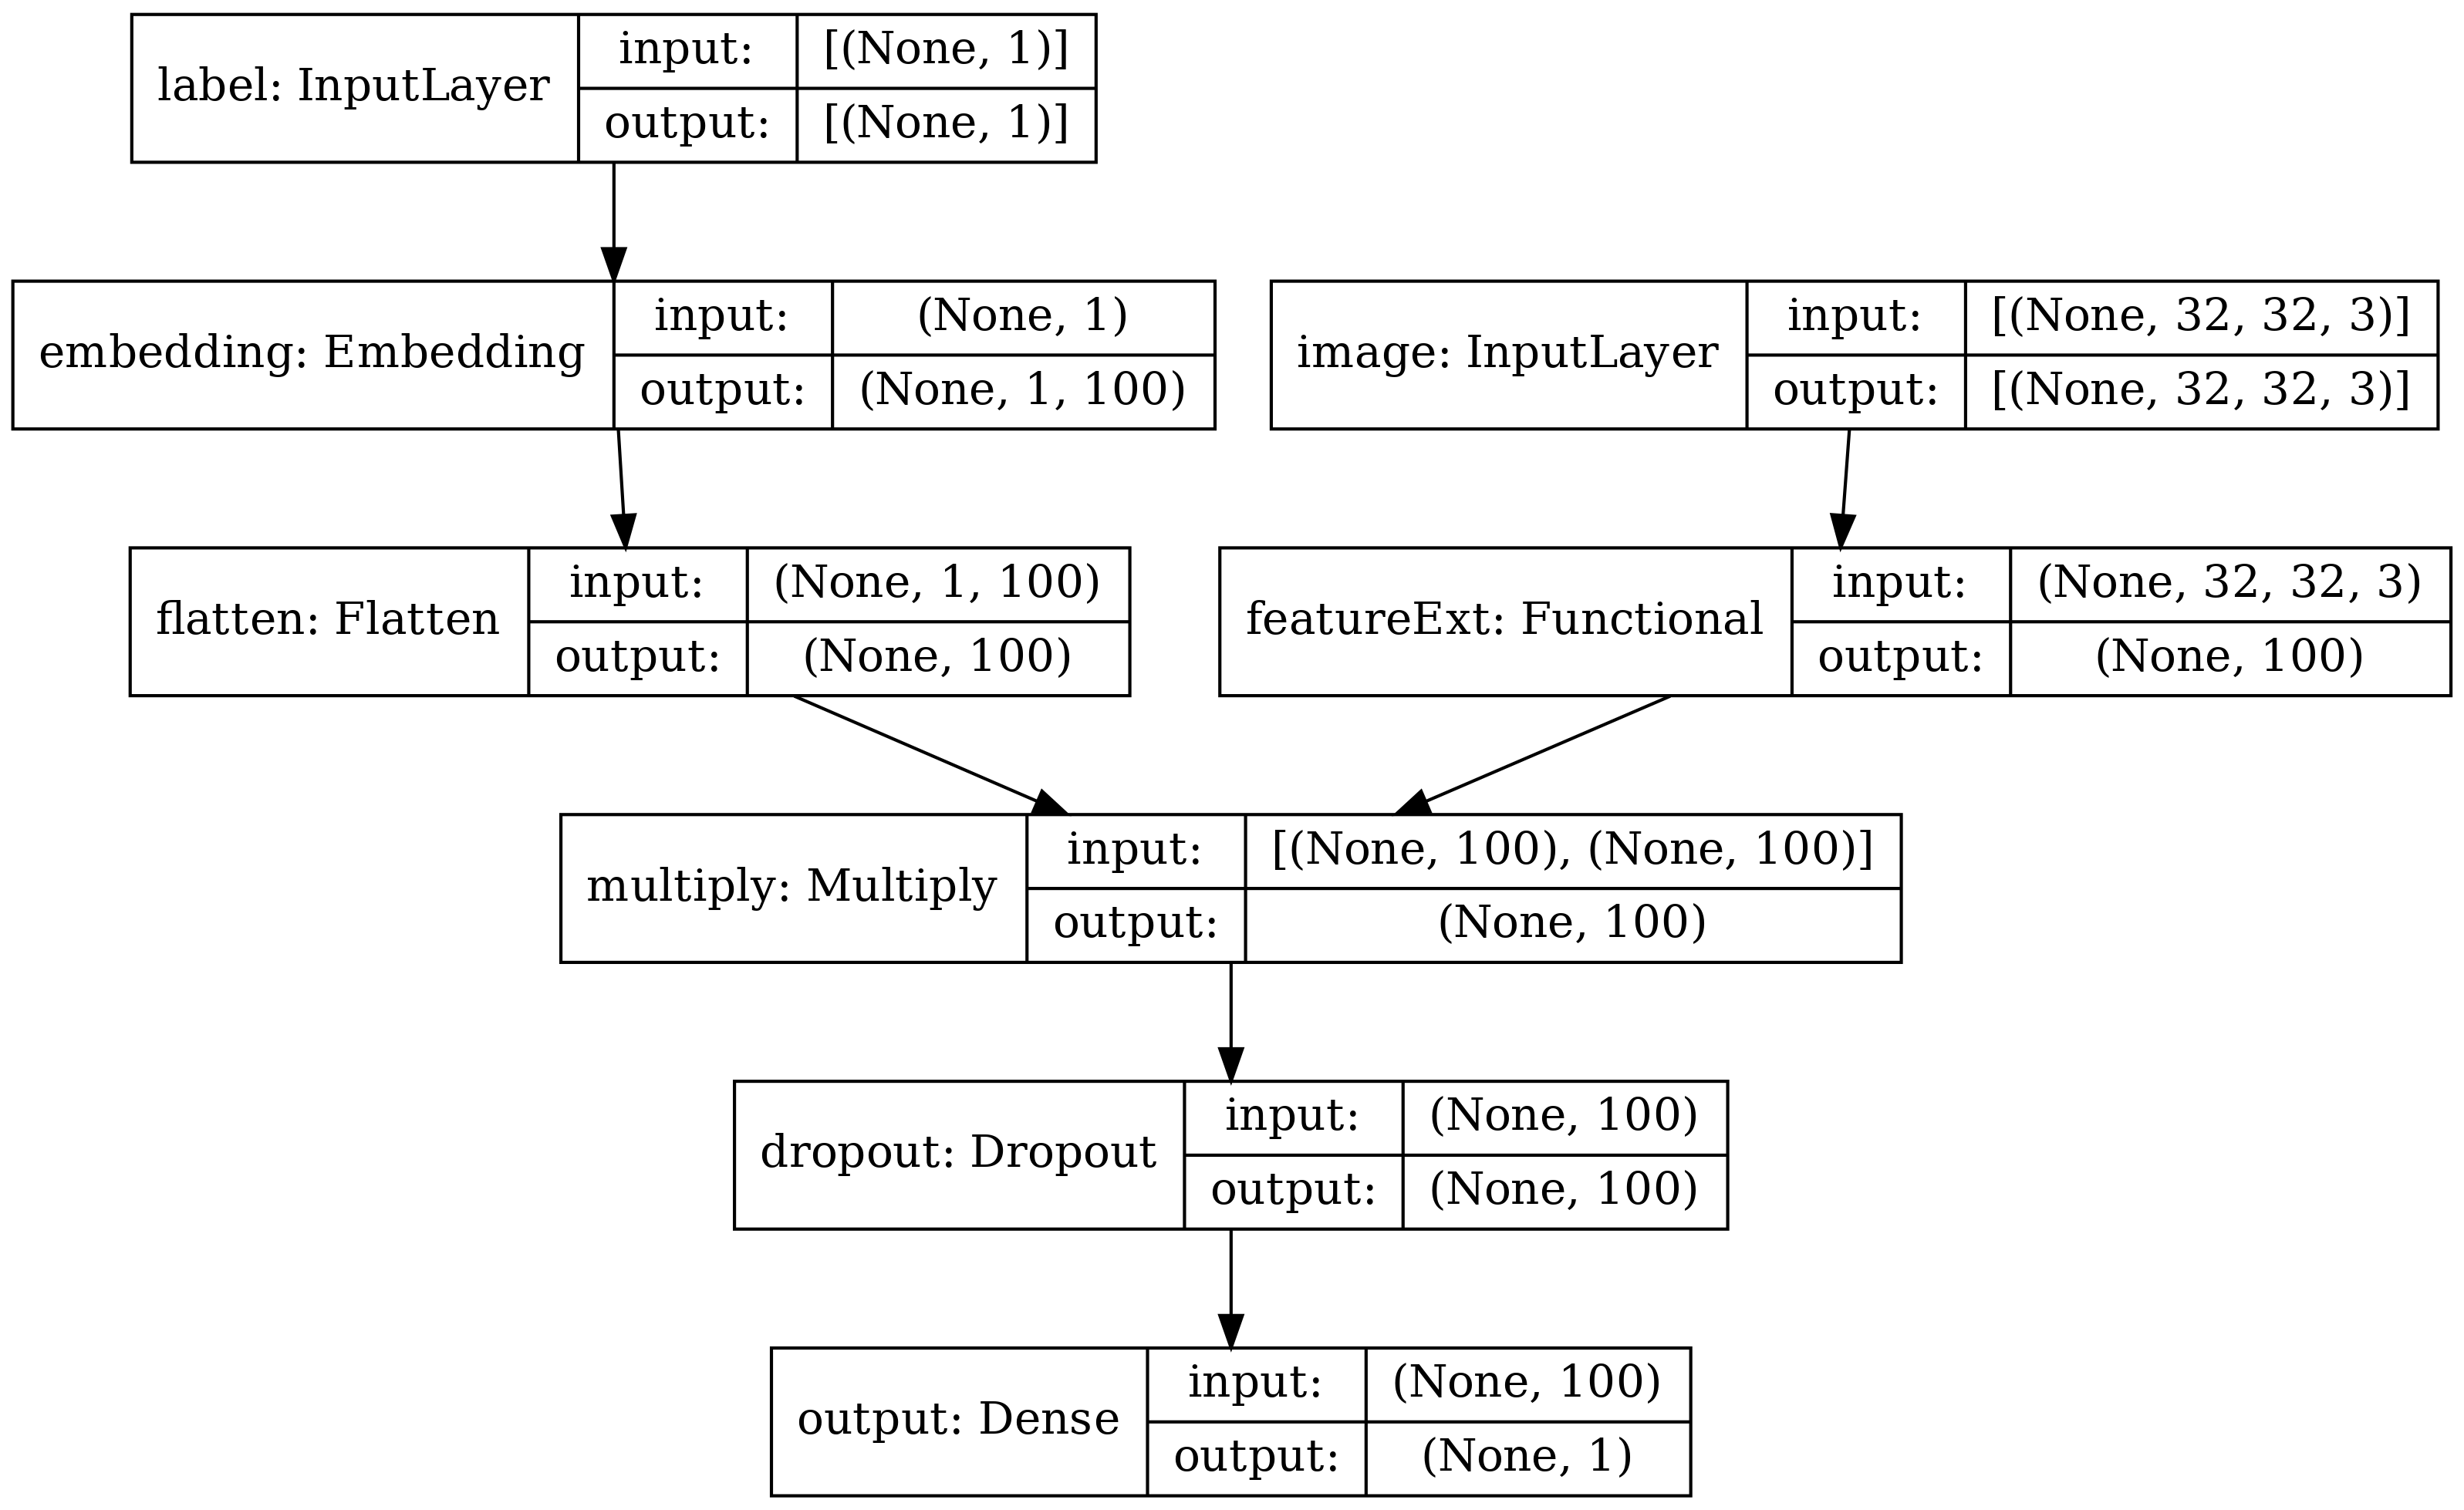
\includegraphics[width=13cm]{images/label_discriminator.png}
\caption{A belső reprezentá és a címke összeállítása a diszkriminátorban}
\label{fig:labeldiscriminator}
\end{figure}

A betanított háló kimeneteire példát a \ref{fig:labelconditioning} ábrán láthatunk, amely a már említett Cifar-10 adathalmaz 10 darab osztályára tanult be. A tanítás során megfigyeltem, hogy az osztályokon belül jelentkezik a mode-collapse jelensége, amely a regularizációs technikák alkalmazása mellett kordábantartható. Illetve a bemeneti zajvektor dimenziójának növelésével is némileg később jelentezett a mode-collapse, viszont egy ilyen kisebb példánál, 32x32-es felbontás mellett nem indokolt az 512 dimenziójú zajvektor használata, így ez nem tekinthető megoldásnak a mode-collapse, hiszen a modellek paramétereinek száma is megnövekedett a GAN-ban.

\begin{figure}[h]
\centering
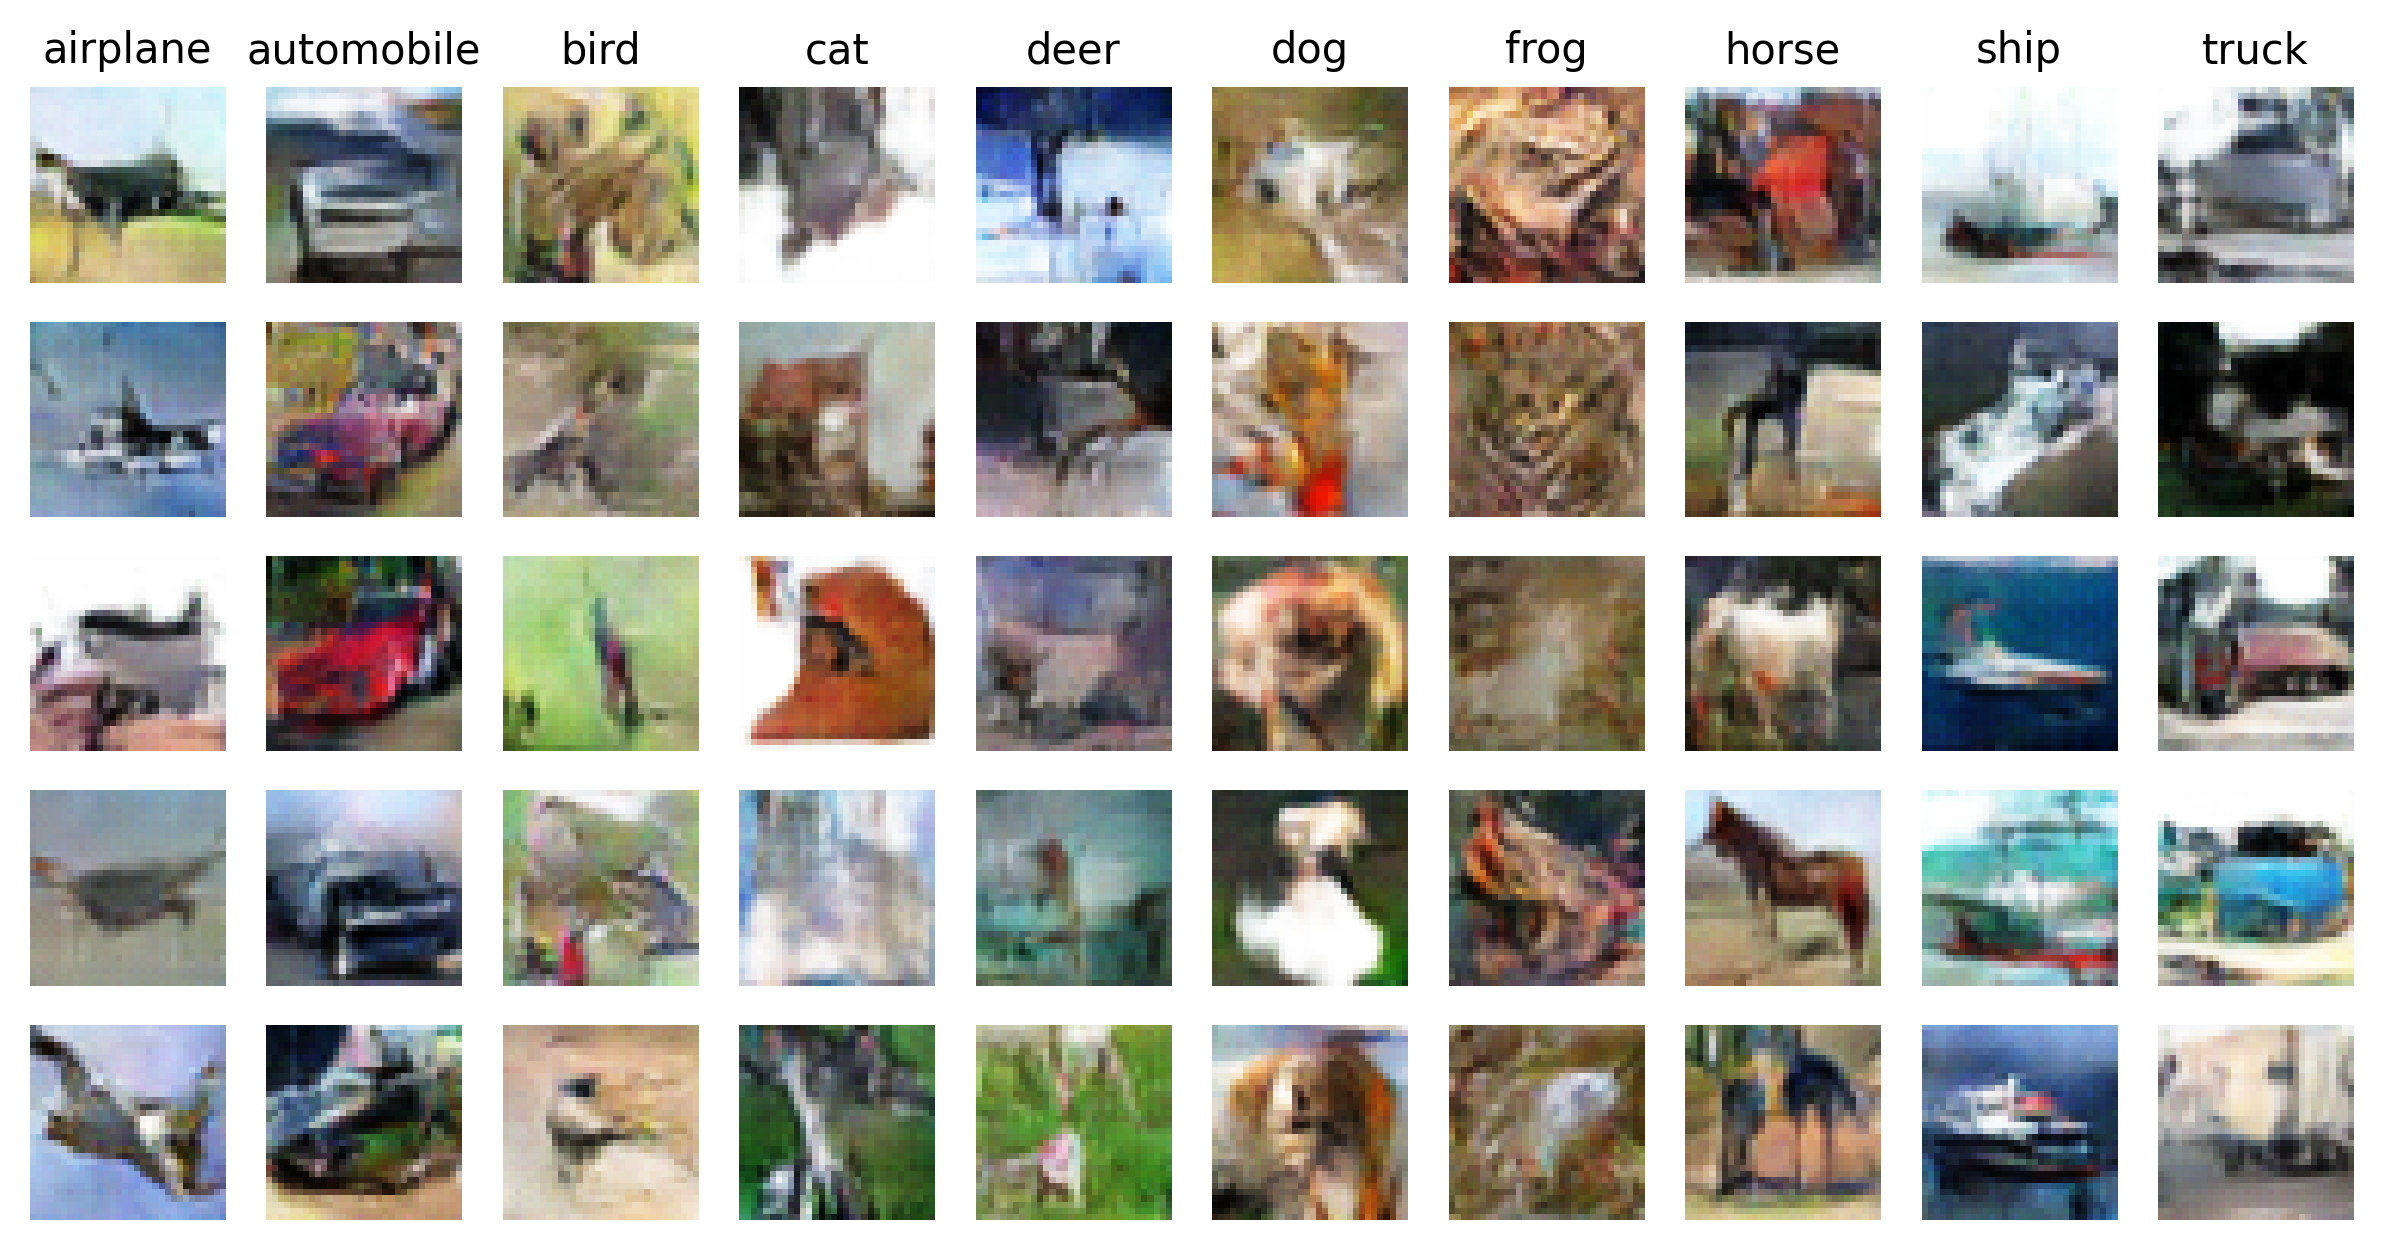
\includegraphics[width=13cm]{images/label_conditioning.png}
\caption{Label conditioning tecnikával tanított Generátor kimenetei}
\label{fig:labelconditioning}
\end{figure}